\section{Visual Design}

\subsection{Event}
An event is represented by a rounded rectangle with a short text inside summarizing its content. The width of the event rectangle is constrained by a threshold and long text is trimmed to fit into its area. The full content of an event will be revealed when it is mouse hovered. Events can be classified into different categories based on certain criteria. For example, a news article may write about \emph{sport}, \emph{fashion} or both. Small colored badges are added to the left of the text of an event to indicate its categories. However, only around 12 colors can be distinguished simultaneously in the human view~\cite{Munzner2014}. Therefore, only the eight most frequently appeared categories are displayed using a given colormap (chosen from Qualitative Set 1 of  ColorBrewer~\cite{Harrower2003}); whereas, the rest share another color. \autoref{fig:event} shows an event with three categories.

Events are shown along and above a horizontal time axis, consisting of two hierarchical temporal scales, which are changed dynamically according to the range of the visible events. For example, the time axis in \autoref{fig:sl-overview} shows \emph{month} and \emph{day}, but they can be switched to \emph{year} and \emph{month} to cover the range of events if needed. An event rectangle is left-aligned with its temporal value on the time axis. To reduce cluttering, an event is not visually connected to its corresponding time point on the axis: it only appears when the event is hovered. This visual design of events satisfies the Technical Requirement 1 -- event representation.

\subsection{Schema}
\label{sub:schema}

\begin{figure}
\centering
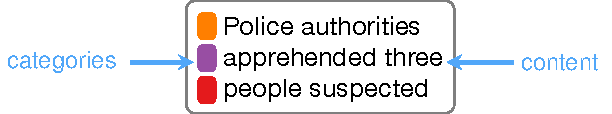
\includegraphics[width=0.75\linewidth]{event}
\caption[Visual representation of an event]{Visual representation of an event. Text shows the content and colored badges indicate the categories.}
\label{fig:event}
\end{figure}

A schema is considered as a sequence of related events. To visualize the connection between events within the same schema effectively, Gestalt principles of grouping are commonly used. The most effective ones are \emph{connectedness} and \emph{proximity} as discussed in the Literature Review chapter. Therefore, we also apply these two principles in our design: events belonging to the same schema are located close together, and the background of an entire schema is colored to visually connected all of its events. Spatial grouping needs to be achieved through vertical positioning because the horizontal position of each event is already determined by its temporal information. Locating all events within a schema close together also makes it convenient to follow them chronologically, addressing Technical Requirement 2 -- schema layout.

Munroe's hand-drawn movie narrative charts~\cite{Munroe2009} show the dynamic interactions of characters throughout the movie. Each character is represented as a curved line along a horizontal time axis; and vertical grouping of lines indicates which characters are together at a given interval. Inspired by this technique, we consider a schema as a ``character line'', connecting all of its events. However, instead of a thin line, we use a thicker path to provide enough space for displaying the content of events and to allow convenient interaction with individual events. For aesthetics, the path is connected rectilinearly, including only horizontal and vertical segments. Also, all events are constrained by the same height to make the width of the path consistent. \autoref{fig:schema} shows two examples of schema.

\begin{figure}
	\centering
	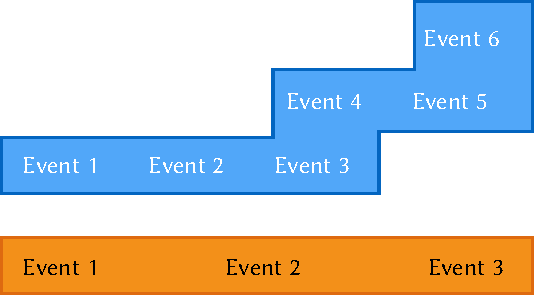
\includegraphics{schema}
	\caption[Visual representation of a schema]{Visual representation of a schema as a colored stripe. Bottom: a simple rectangle connects events that can display in the same row. Top: a rectilinear path connects events that need to locate in different rows.}
	\label{fig:schema}
\end{figure}

Putting it all together, \autoref{fig:sl-overview} shows a complete example of SchemaLine visualization. \autoref{sec:sl-algorithm} discusses how to produce such a visualization.

\begin{figure}
	\centering
	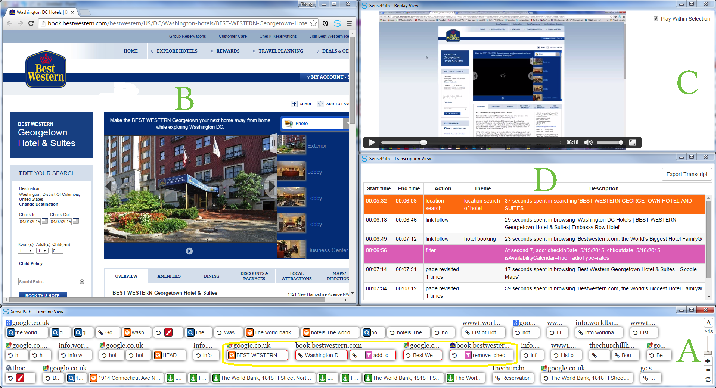
\includegraphics[width=\linewidth]{overview}
	\caption[SchemaLine visualization of events]{SchemaLine visualization of events; related ones are connected into schemas. Note that events are duplicated if they belong to multiple schemas.}
	\label{fig:sl-overview}
\end{figure}

\subsection{Interaction for Externalizing Sensemaking}
To enable analysts to intuitively perform sensemaking activities through interaction (Technical Requirement 3 -- Data--Frame model), we follow the design guidelines of fluid interaction proposed by Elmqvist~et~al.~\cite{Elmqvist2011}. More specifically, SchemaLine
\begin{itemize}
	\item Produces smooth animated transitions between the state before and the state after an interaction, helping analysts maintain their mental maps.
	\item Provides immediate visual feedback, enabling analysts to beware of what is happening and/or what will happen next.
	\item Allows direct manipulation on the visual representations of events and frames, instead of using extra menus and buttons.
\end{itemize}

During sensemaking, when an analyst recognizes a relationship of events, he or she may group them together and find an account for them (\textbf{connect data and a frame}). This activity can be performed by dragging one event and dropping it onto another event, producing a new frame consisting of these two. While dragging over, a \emph{plus} icon and a rectangle with dashed border surrounding the two events are displayed to indicate that a new frame will be created.

The analyst may also want to \textbf{elaborate the frame} by adding more relevant events into it. This can be simply executed by dropping events onto the colored stripe representing the frame. Conversely, to \textbf{preserve the frame}, the analyst can drag its events and drop them onto void space to remove them from the frame. Appropriate informative feedback is displayed in both cases: a \emph{plus} icon for elaboration and a \emph{minus} icon for preservation. \autoref{fig:add-event-frame} shows an example for elaborating the frame.

\begin{figure}
	\centering
	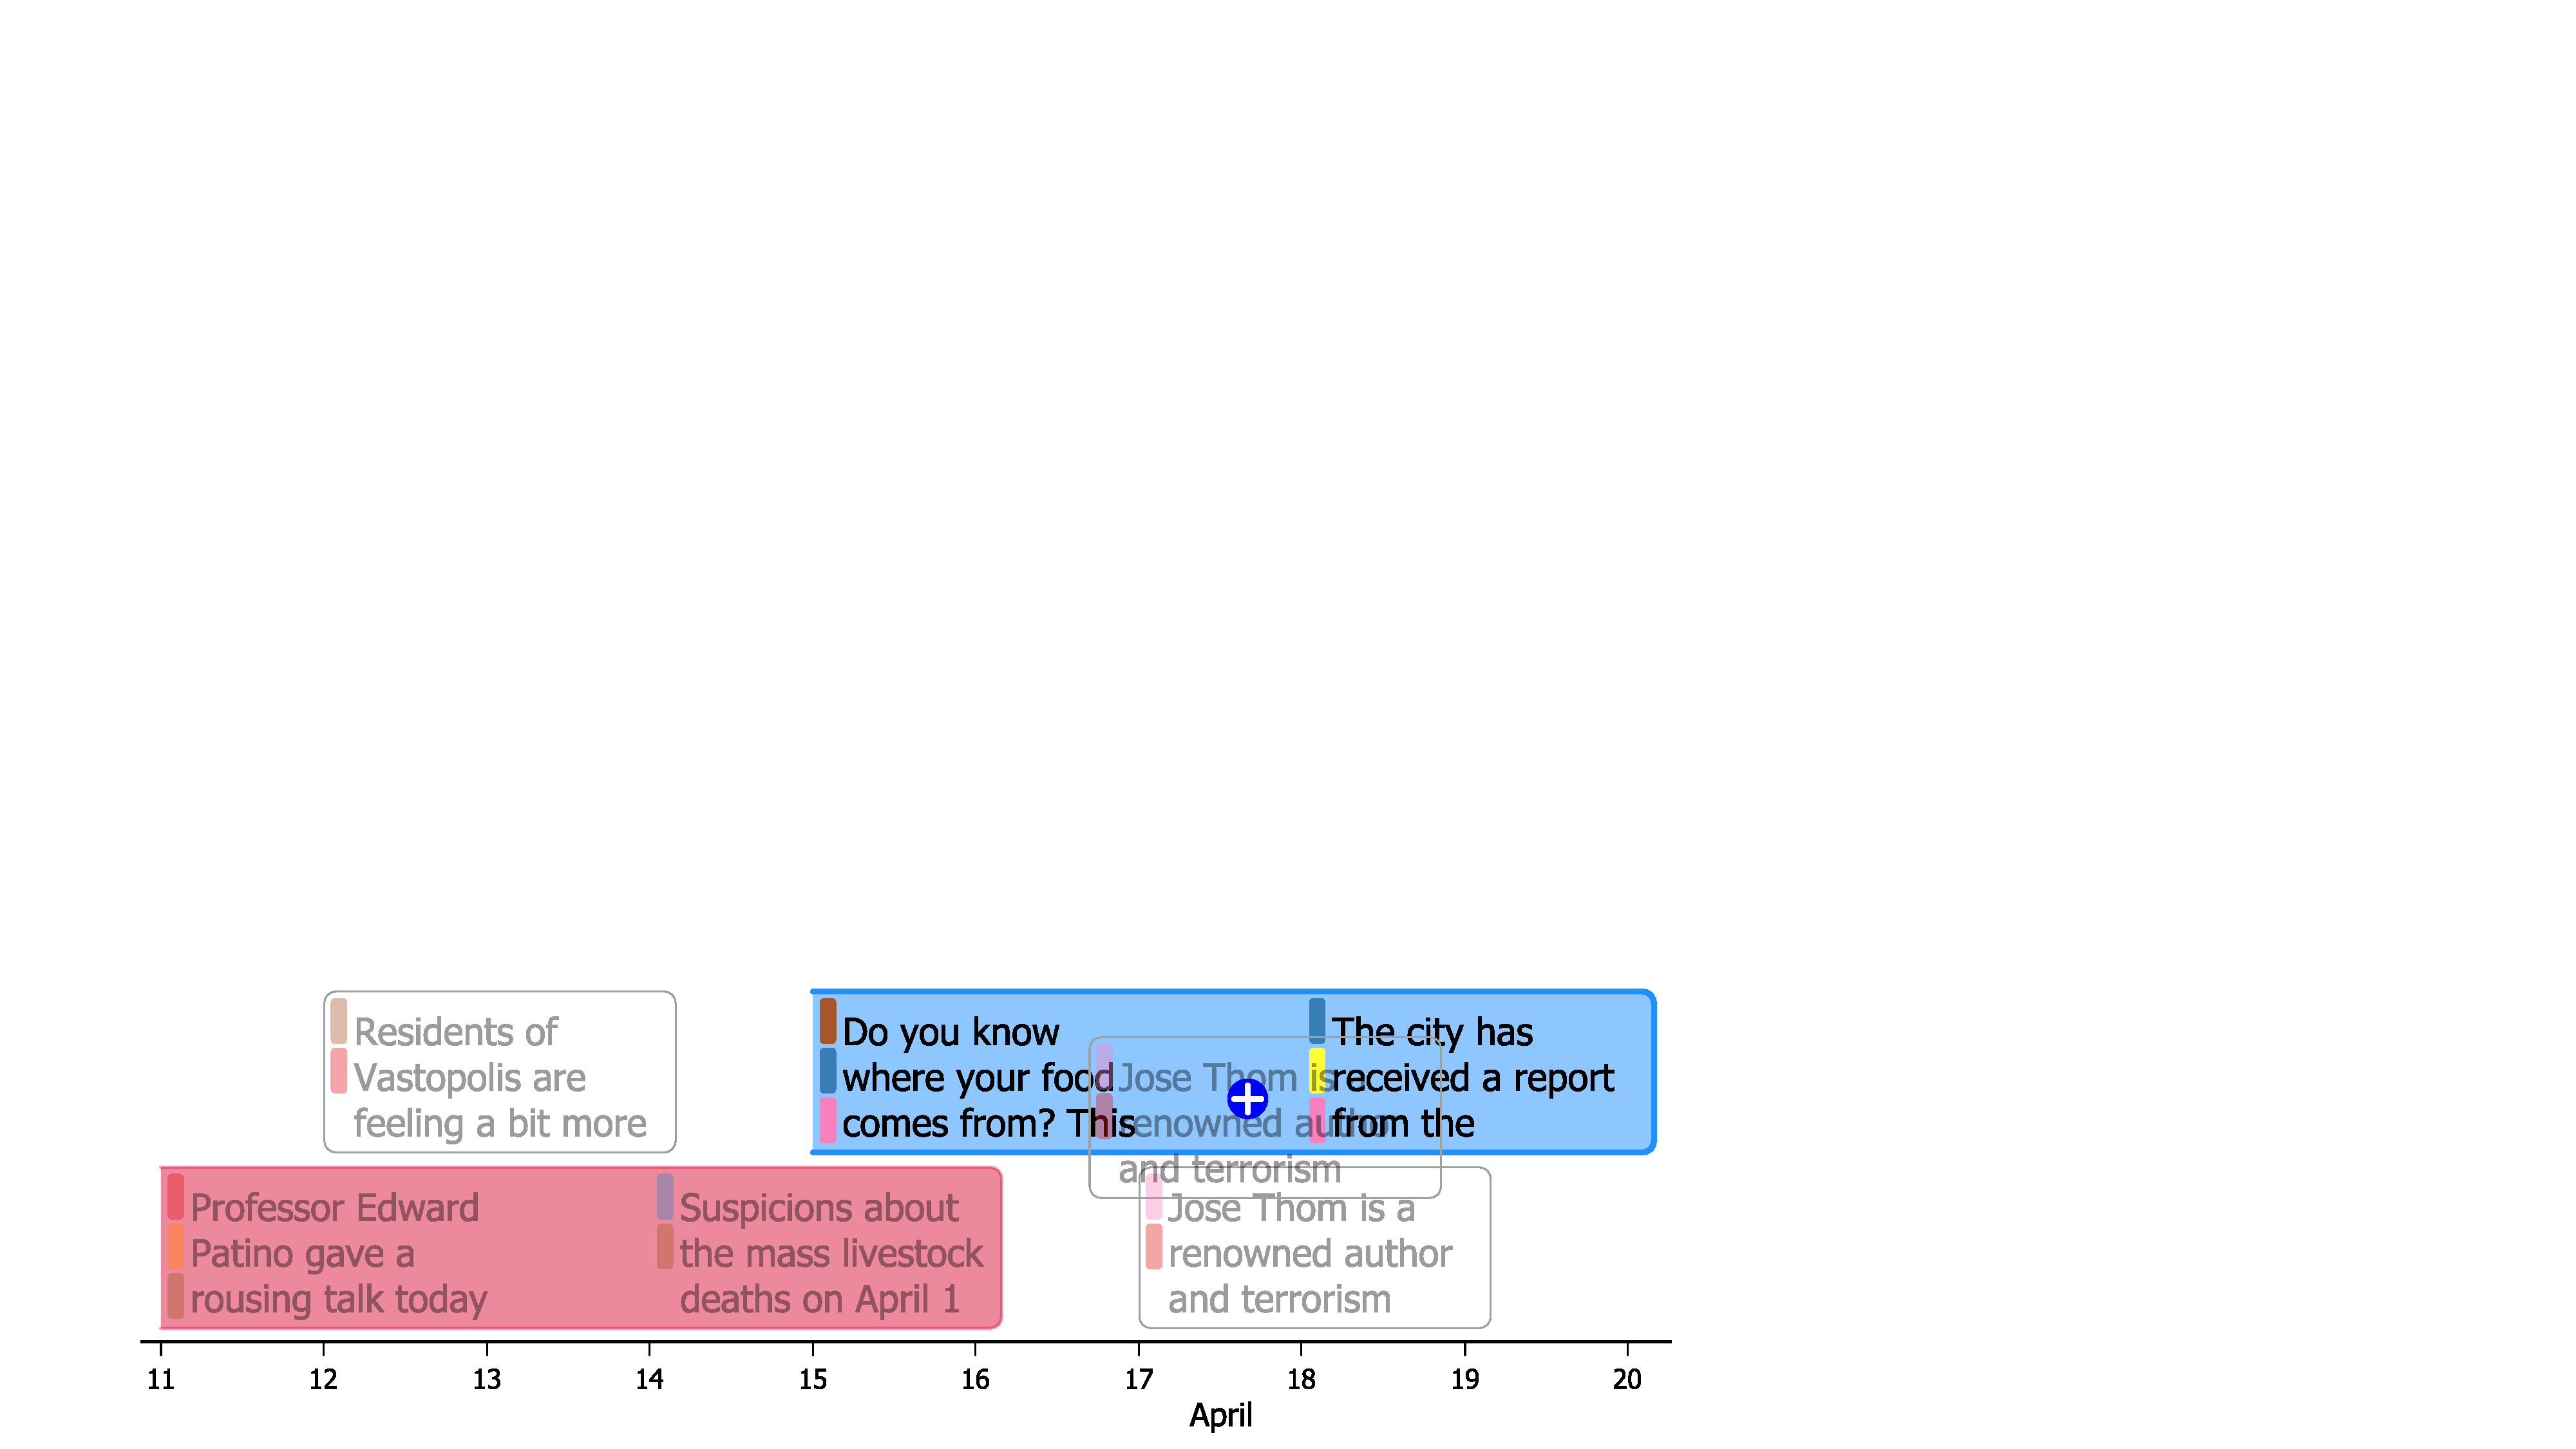
\includegraphics[width=\linewidth]{add-event-frame}
	\caption[Elaborating the frame]{Elaborating the frame. Dragging and dropping an event onto the blue stripe to add it to that frame. The plus icon indicates the additional behavior of dropping the event.}
	\label{fig:add-event-frame}
\end{figure}

\textbf{Questioning the frame} occurs when the analyst encounters inconsistencies in the data. The temporal distribution of events in the frame may raise concerns about the plausibility and completeness of the frame. For example, if a frame about one person contains many events in January and March, but none in February; it may be inferred that some data might be missed. To highlight a suspected event, the analyst can double-click on it with the right mouse button. The text of that event will be rendered in red to bookmark that it requires further investigation.

Depending on experience, the analyst can think of multiple explanations for the same set of data. To support \textbf{comparing multiple frames}, we enable the analyst to duplicate events and construct similar frames. By default, dragging an event from one frame and dropping it onto another frame will move it to the new frame. However, holding the \emph{Control} key while dropping an event will instead copy it to the new frame. Also, when two frames are selected, they will be moved vertically next together to facilitate comparison.

The analyst can remove an event from the timeline by dropping it at the bottom of the time axis. A red \emph{remove} icon is displayed as a visual feedback. While searching for a replacement to account for inconsistent and contrary data (\textbf{reframing}), it could be useful to consider discarded data. To enable that, SchemaLine can redisplay events that were removed earlier with half transparency to distinguish them from existing events.

When the analyst thinks that the existing frame cannot account for its data, he or she may  completely discard it and \textbf{seek a new frame}. The frame can be removed by dropping it onto void space. However, its events still remain in the timeline, enabling the analyst to exploit them. Another interaction could be useful is to combine two sets of events together -- we call it ``merge frames''. This can be performed by dragging one schema and dropping it on top of the other schema.